\section{Related Experimental Results}
\label{sec:introduction:relatedWorks}

This section gives a brief review of two groups of related experiments: the LU tests in the charged weak decays and the measurements of \absVcs.

\subsection{Tests of Lepton Universality}
\label{sec:introduction:relatedWorks:lu}


\subsubsection{Test with \PW Boson Decay} 
~
% Test with \PW boson decay can be summarized into three eras: 1) SPS and Tevatron, 2) LEP, 3) LHC.




% SPS and Tevatron Experiments
\underline{SPS and Tevatron}

Both SPS and Tevatron collide protons and anti-protons. SPS operated at CERN from 1981 to 1991 at a center-of-mass energy of 0.546\TeV and 0.630\TeV. The SM electroweak bosons, \PW and \PZ, were first discovered in the SPS in 1983 \cite{ARNISON1983103, BANNER1983476}. In 1985, Tevatron at Fermilab began operations at a higher center-of-mass energy at 1.8\TeV, which was later upgraded to 1.96\TeV in its second run since 2001. Tevatron was in service for more than 20 years until 2010 to give ways to the LHC. 
% The properties of the weak bosons were measured with higher precision by Tevatron experiments. 


\begin{figure}[ht]
    \centering
    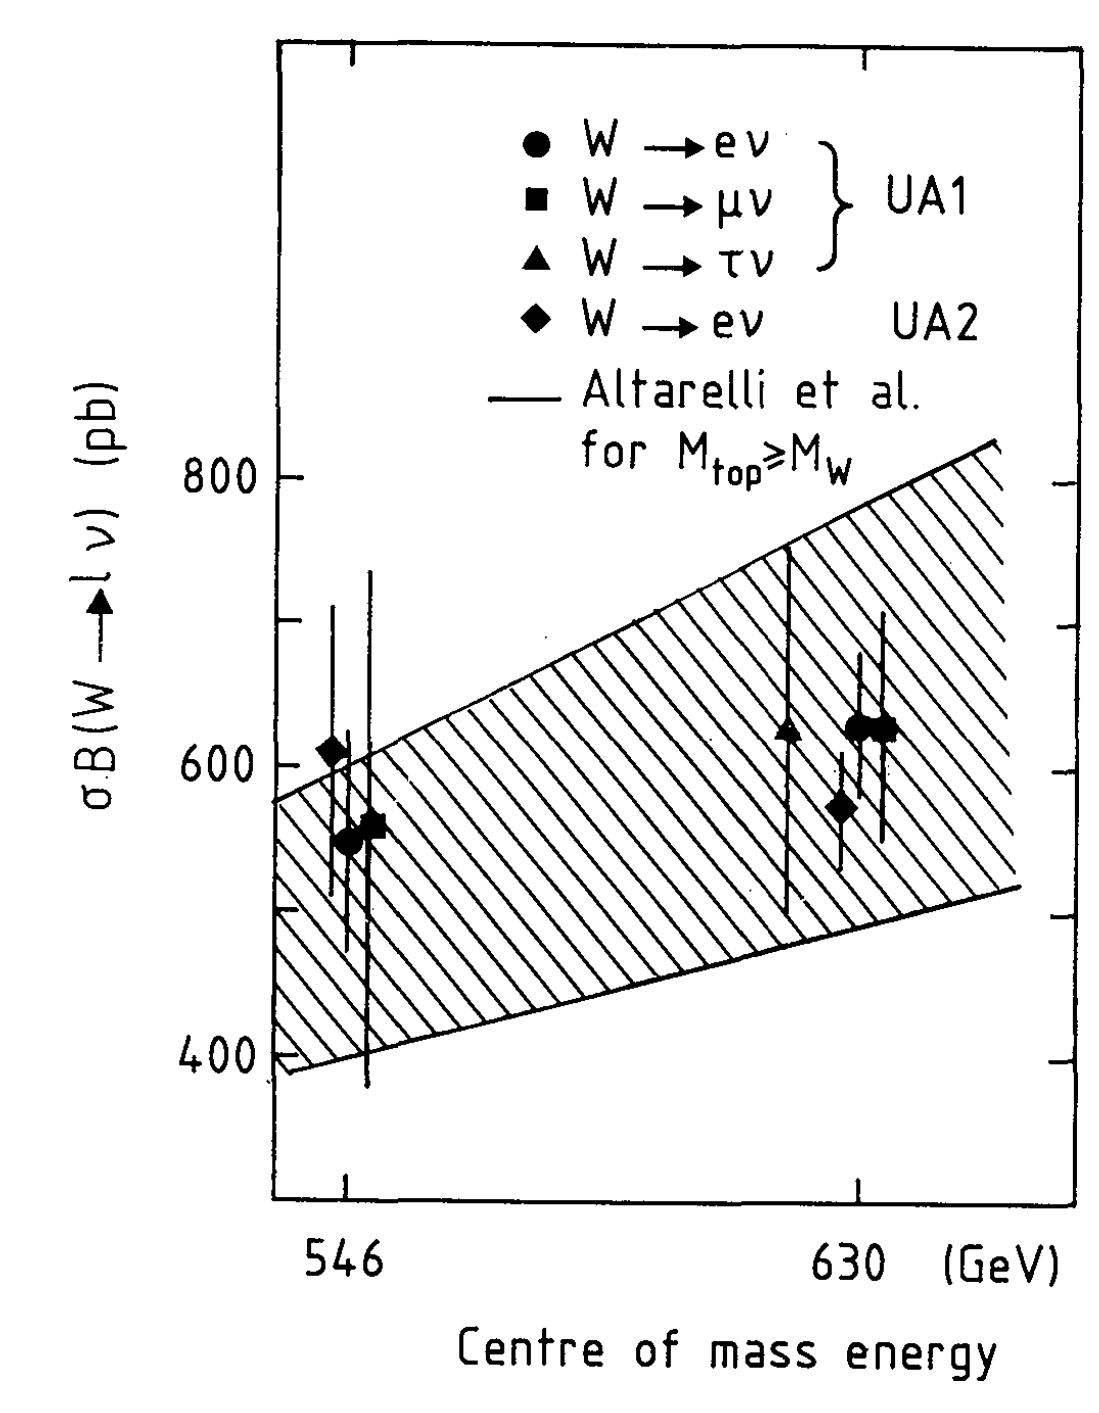
\includegraphics[height=0.35\textheight]{chapters/introduction/sectionRelatedWorks/figures/sps.png} \qquad
    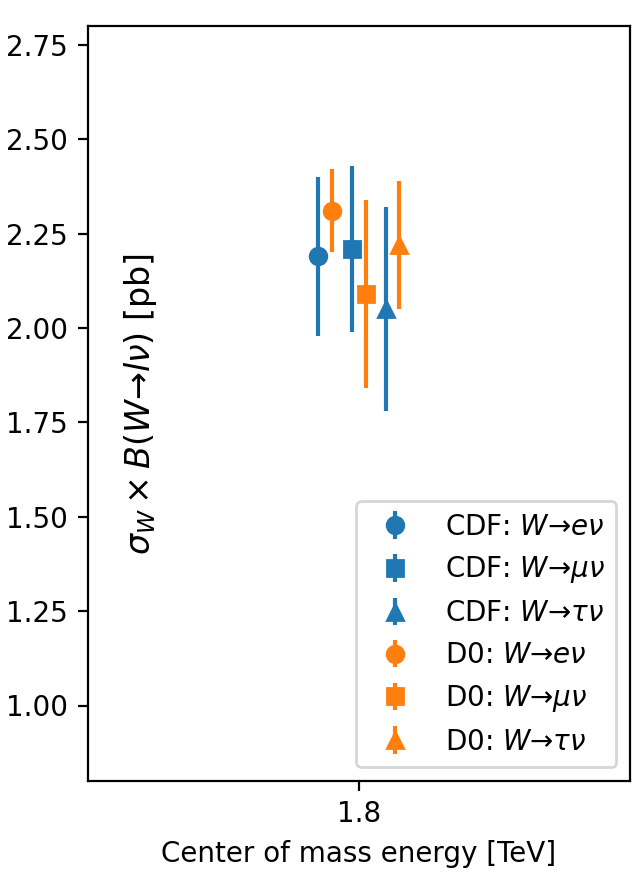
\includegraphics[height=0.35\textheight]{chapters/introduction/sectionRelatedWorks/figures/tevatron.png}
    \caption{Measurement of $\sigma_{\Pp\bar{\Pp}\to \PW} \times \BWl$ for $\ell \in \{ \Pe, \PGm, \PGt\}$ by the SPS \cite{Albajar:1988ka} and Tevatron~\cite{Abazov:2003sv, Abbott:1999tt, Abachi:1995xc, Abbott:1999pk, Abe:1990sd, Abe:1992ys, Abe:1991fb} experiments.}
    \label{fig:introduction:relatedWorks:spsTevatron}
\end{figure}


% SPS Tevatron result plot
\begin{figure}[ht]
    \centering
    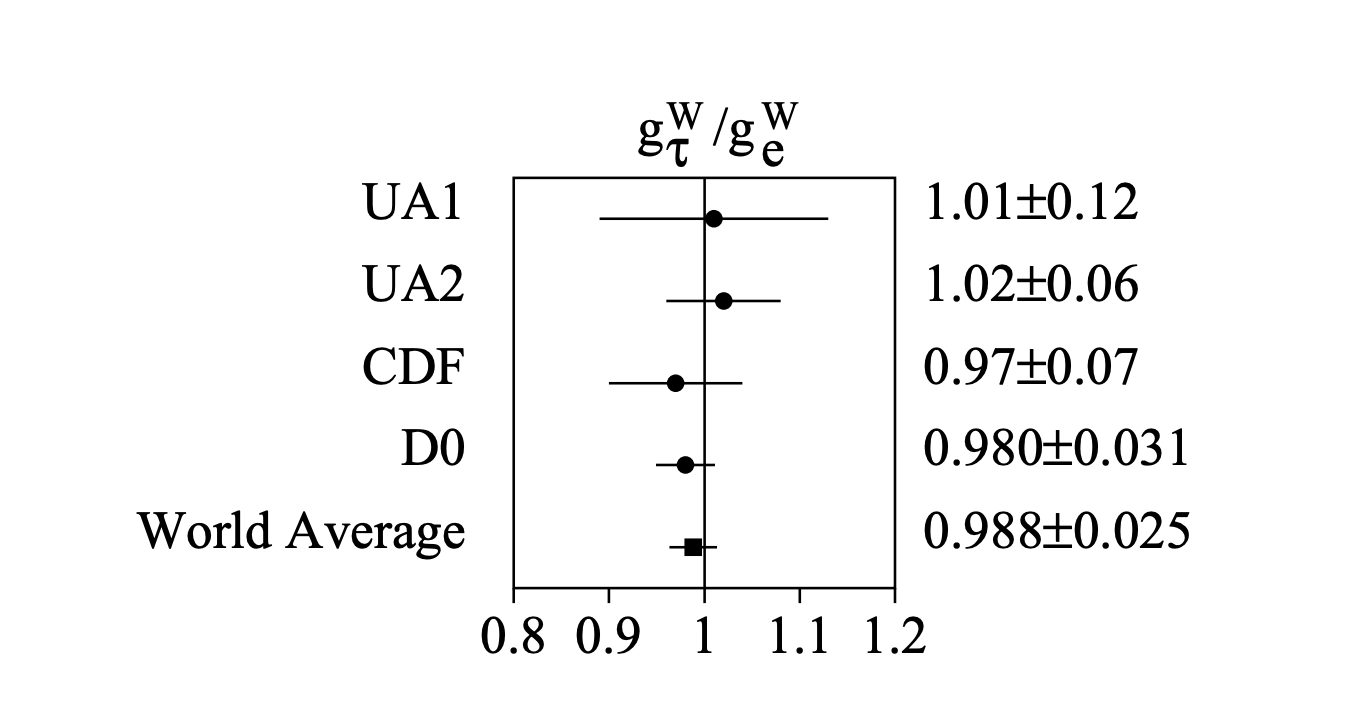
\includegraphics[width=0.5\textwidth]{chapters/introduction/sectionRelatedWorks/figures/spsTevatron.png}
    \caption{ $g^\PW_\PGt / g^\PW_\Pe$ measured by the SPS and Tevatron experiments \cite{Abbott:1999pk}. In all the four experiments, the ratio of the weak coupling constant between electron and tau was extracted by the ratio of $\sigma_{\Pp\bar{\Pp}\to \PW} \times \BWt$ and $\sigma_{\Pp\bar{\Pp}\to \PW} \times \BWe$. The average was combined by \DZERO collaboration~\cite{Abbott:1999pk}, the last published result among the four.}
    \label{fig:introduction:relatedWorks:spsTevatronCombinedRatio}
\end{figure}


The UA1, UA2 at the CERN SPS and the CDF, \DZERO at the Fermilab Tevatron measured $\sigma_{\Pp\bar{\Pp}\to \PW} \times \BWl$ for $\ell \in \{ \Pe, \PGm, \PGt\}$, shown in Figure~\ref{fig:introduction:relatedWorks:spsTevatron}. The LU test is performed by taking the ratios of two different leptonic channels. Figure~\ref{fig:introduction:relatedWorks:spsTevatronCombinedRatio} from \cite{Abbott:1999pk} summarizes the results of $g^\PW_\PGt / g^\PW_\Pe$ derived by the SPS and Tevatron experiments. The combined average was calculated by the \DZERO collaboration~\cite{Abbott:1999pk}, which was the last published result among the four. The average assumed uncorrelated systematical and statistical uncertainties. All four measurements confirmed consistency with the SM lepton universality within one experimental uncertainty.



% SPS result table
\begin{table}[ht]
    \setlength{\tabcolsep}{ 0.5 em}
    \renewcommand{\arraystretch}{1.5}
    \centering
    \caption{The measurement of $\sigma_{\Pp \bar{\Pp} \to \PW} \times \BWl$ for $\ell \in \{ \Pe, \PGm, \PGt\}$ and the ratios between leptonic channels by UA1 and UA2 at the CERN SPS. }
    \resizebox{\textwidth}{!}{
    \begin{tabular}{ |c|l l| } 
         
         % UA1 result
         \hline
         \multicolumn{3}{|c|}{UA1 \cite{Albajar:1988ka} }  \\
         \hline
         & $\Pp \bar{\Pp}$ at $\sqrt{s}=0.546$ TeV &  $\Pp \bar{\Pp}$ at $\sqrt{s}=0.630$ TeV \\
         \hline
         $\sigma_{\Pp \bar{\Pp} \to \PW} \times \BWe$  [nb]  & 0.55 $\pm$ 0.08 (stat) $\pm$ 0.09 (syst) & 0.63 $\pm$ 0.06 (stat) $\pm$ 0.10 (syst) \\ 
         $\sigma_{\Pp \bar{\Pp} \to \PW} \times \BWm$  [nb]  & 0.56 $\pm$ 0.18 (stat) $\pm$ 0.12 (syst) & 0.63 $\pm$ 0.08 (stat) $\pm$ 0.11 (syst) \\ 
         $\sigma_{\Pp \bar{\Pp} \to \PW} \times \BWt$  [nb]  & \multicolumn{2}{c|}{ 0.63 $\pm$ 0.13 (stat) $\pm$ 0.12 (syst) }  \\ 
         \hline
         $\BWm / \BWe$  & \multicolumn{2}{c|}{1.00  $\pm$ 0.14 (stat) $\pm$ 0.08 (syst) } \\
         $\BWt / \BWe$  & \multicolumn{2}{c|}{1.02  $\pm$ 0.20 (stat) $\pm$ 0.10 (syst) } \\
         
         \hline
         \multicolumn{2}{c}{} \\
         
         % UA2 result
         \hline
         \multicolumn{3}{|c|}{UA2}  \\
         \hline
         & $\Pp \bar{\Pp}$ at $\sqrt{s}=0.546$ TeV &  $\Pp \bar{\Pp}$ at $\sqrt{s}=0.630$ TeV \\
         \hline
         $\sigma_{\Pp \bar{\Pp} \to \PW} \times \BWe$  [nb] \cite{appel1986measurement} & 0.50 $\pm$ 0.09 (stat) $\pm$ 0.05 (syst) & 0.53 $\pm$ 0.06 (stat) $\pm$ 0.05 (syst) \\ 
         % This is UA2 result reported in the UA1 summary
        %  $\sigma_W \times Br(W\to e    \nu)$  [nb] \cite{Albajar:1988ka} & 0.61 $\pm$ 0.10 (stat) $\pm$ 0.07 (syst) & 0.57 $\pm$ 0.04 (stat) $\pm$ 0.07 (syst) \\ 
         \hline
         $\BWt / \BWe$ \cite{Alitti:1992hv} & - & 1.04  $\pm$ 0.08 (stat) $\pm$ 0.08 (syst) \\
         
         \hline
    \end{tabular}}
    \label{tab:introduction:relatedWorks:sps}
\end{table}




% Tevatron result table
\begin{table}[ht]
    \setlength{\tabcolsep}{0.5 em}
    \renewcommand{\arraystretch}{1.5}
    \centering
    \caption{The measurement of $\sigma_{\Pp \bar{\Pp} \to \PW} \times \BWl$ for $\ell \in \{ \Pe, \PGm, \PGt\}$ and the ratios between leptonic channels by CDF and \DZERO at the Fermilab Tevatron.}
    % \resizebox{0.95\textwidth}{!}{
    \begin{tabular}{ |c|l| } 
         

         
         %  CDF result
         \hline
         \multicolumn{2}{|c|}{CDF with $\Pp \bar{\Pp}$ at $\sqrt{s}=1.8$ TeV} \\
         \hline
         $\sigma_{\Pp \bar{\Pp} \to \PW} \times \BWe$  [nb] \cite{Abe:1990sd}    & 2.19 $\pm$ 0.04 (stat) $\pm$ 0.21 (syst) \\ 
         $\sigma_{\Pp \bar{\Pp} \to \PW} \times \BWm$  [nb] \cite{Abe:1992ys}    & 2.21 $\pm$ 0.07 (stat) $\pm$ 0.21 (syst) \\ 
         $\sigma_{\Pp \bar{\Pp} \to \PW} \times \BWt$  [nb] \cite{Abe:1991fb}    & 2.05 $\pm$ 0.27 \\ 
         \hline
         $\BWm / \BWe$ \cite{Abe:1992ys} & 1.02  $\pm$ 0.08 \\
         $\BWt / \BWe$ \cite{Abe:1991fb} & 0.94  $\pm$ 0.14 \\

         \hline
         
         \multicolumn{2}{c}{}  \\
         
         % D0 result
         \hline
         \multicolumn{2}{|c|}{D0 with $\Pp \bar{\Pp}$ at $\sqrt{s}=1.8$ TeV} \\
         \hline
         $\sigma_{\Pp \bar{\Pp} \to \PW} \times \BWe$  [nb] \cite{Abbott:1999tt} & 2.31 $\pm$ 0.01 (stat) $\pm$ 0.05 (syst) $\pm$ 0.10 (lum) \\ 
         $\sigma_{\Pp \bar{\Pp} \to \PW} \times \BWm$  [nb] \cite{Abachi:1995xc} & 2.09 $\pm$ 0.23 (stat) $\pm$ 0.11 (syst) \\ 
         $\sigma_{\Pp \bar{\Pp} \to \PW} \times \BWt$  [nb] \cite{Abbott:1999pk} & 2.22 $\pm$ 0.09 (stat) $\pm$ 0.10 (syst) $\pm$ 0.10 (lum)  \\ 
         \hline
         $\BWm / \BWe$ \cite{Abachi:1995xc} & 0.89  $\pm$ 0.10 \\
         $\BWt / \BWe$ \cite{Abbott:1999pk} & 0.961 $\pm$ 0.061 \\
         
         \hline
         
         
    \end{tabular}
    % }
    \label{tab:introduction:relatedWorks:tevatron}
\end{table}


UA1 was a general-purpose particle detector at the CERN SPS, consisting of the inner tracker, electromagnetic calorimeter, hadronic calorimenter, and a muon system, sequentially from the inside to the outside.  It took 0.546\TeV and 0.63\TeV data during 1982-1983 and 1984-1985, respectively.  Its \PW boson measurement is summarized in \cite{Albajar:1988ka}.  $\PW \to e \PGn$ events were selected based on single electron plus missing transverse energy (\MET). The QCD and $\PW\to \PGt_\Pe \PGn$ background were estimated by the data-driven approach and simulation, respectively. In total, 59 and 240 $\PW \to e \PGn$ events were selected from the 0.546\TeV and 0.63\TeV dataset, respectively.  $\PW \to \PGm \PGn$ events were selected based on single muon plus \MET trigger. The background involving muons from tau and meson decays was estimated by simulations. In total, 10 and 57 $\PW\to \PGm\PGn$ events were selected from 0.546\TeV and 0.63\TeV dataset.  $\PW\to \PGt \PGn$ sample was selected with a single hadronic tau plus \MET selection. The hadronic taus were identified as highly collimated narrow jets with low charged-track multiplicities.  A $\PGt$-likelihood was calculated for each jet candidate based on the its shape and charged tracks. In total, 32 events were selected from the combined 0.546\TeV and 0.63\TeV dataset. Based on the yields, UA1 reported the $\sigma_{\Pp\bar{\Pp}\to \PW} \times \BWl$ for $\ell \in \{ \Pe, \PGm, \PGt\}$ at 0.546\TeV and 0.63\TeV center-of-mass energy. Pair-wise ratios were calculated to test the lepton universality. Table~\ref{tab:introduction:relatedWorks:sps} lists the measurements by UA1.



UA2 was a particle detector at the CERN SPS, consisting of a tracking system surrounded by a calorimetry system with electromagnetic and hadronic compartments. Unlike UA1, UA2 was not a multipurpose detector; its focus was on the calorimeters and did not have a muon detector. Therefore, lepton universality test on UA2 mainly involved the $\PW \to e\PGn$ and $\PW \to \PGt \PGn$. \cite{appel1986measurement} summarized the $\sigma_{\Pp\bar{\Pp}\to \PW} \times \BWe$ measurements from the UA2 using 0.546 TeV and 0.63 TeV dataset collected during 1982-1983 and 1984-1985. The measurement was based on single-electron plus \MET trigger. After the UA2 upgrade during 1985-1987, tau channel was added and a test of the lepton universality between electrons and taus was performed \cite{Alitti:1991eh, Alitti:1992hv}, using the 0.63 TeV data collected during 1988-1990. The hadronic taus were reconstructed from jet candidates with requirements on the relative hadronic energy and the lateral energy profile. The data was triggered with \MET trigger in 1988-1989 and a dedicated hadronic tau trigger in 1990. \cite{Alitti:1991eh} analyzed the former dataset, while \cite{Alitti:1992hv} combined the two datasets. The result \cite{Alitti:1992hv} for the ratio between tauonic decay and electronic decay is shown in the Table~\ref{tab:introduction:relatedWorks:sps}. 






CDF was an azimuthally and forward-backward symmetric general-purpose detector at the Fermilab Tevatron. It was consist of several subdetector layers, including a silicon tracker, a gas chamber as the central outer tracker, solenoid magnet, electromagnetic and hadronic calorimeters, and muon detector. CDF began taking its first data in 1985 and started its run-1 data taking after its first upgrade in 1989. For $\PW \to e  \PGn$, \cite{Abe:1990sd} presented a measurement of $\sigma_{\Pp\bar{\Pp}\to \PW} \times \BWe$ using the single-electron trigger. For $\PW \to \PGm  \PGn$, \cite{Abe:1992ys} presented a measurement of $\sigma_{\Pp\bar{\Pp}\to \PW} \times \BWm$ and the ratio of muon and electron channels. This measurement used the single-muon trigger. Citing the previous CDF result on $\sigma_{\Pp\bar{\Pp}\to \PW} \times \BWe$ \cite{Abe:1990sd}, it obtained the ratio of the muonic and electronic weak coupling as $g^\PW_\PGm/g^\PW_\Pe=1.01\pm0.04$, consistent with the lepton universality. Both electron and muon channels required \MET to target the \wjets events.  For $\PW \to \PGt \PGn$, \cite{Abe:1991fb} measured the $\sigma_{\Pp\bar{\Pp}\to \PW} \times \BWt$ and its ratio to the previously obtained electronic channel \cite{Abe:1990sd}. The tau channel was based on two triggers, \MET trigger and single-tau trigger (presence of a tau jet with a lower threshold of \MET), which yielded 132 and 47 final events respectively. The tau identification required 0-3 tracks with no tracks in the \ang{10} - \ang{30} region separate from the seeding track. Combining the two triggers, the ratio between tau channel and electron channel was reported as $g^\PW_\PGt/g^\PW_\Pe=0.97\pm0.07$, consistent with the SM lepton universality. Table~\ref{tab:introduction:relatedWorks:tevatron} lists the CDF results.



\DZERO was consist of a hybrid tracking system with silicon inner tracker and scintillator fiber outer tracker, superconducting solenoid, electromagnetic and hadronic calorimeter, and muon system. The detector was completed in 1991 and was placed in the Tevatron in February 1992.  \DZERO collected 1.8\TeV data during 1992-1995. With data collected in 1992-1993,  \DZERO presented a measurement of $\sigma_{\Pp\bar{\Pp}\to \PW} \times \BWem$ and their ratio \cite{Abachi:1995xc}. Later, in the year 1994-1995, about 6 times more data was collected, and accordingly $\sigma_{\Pp\bar{\Pp}\to \PW} \times \BWe$ was updated with a better precision \cite{Abbott:1999tt}. It is worth noticing that this update \cite{Abbott:1999tt} also reported the electronic branching fraction as $\BWe=(10.66\pm0.15\pm0.21\pm0.11\pm0.11)\%$, where the uncertainties were for statistics, systematics, theory, and undetermined next-to-leading order theoretical calculation. Also, with the 1994-1995 data,  \DZERO measured $\sigma_{\Pp\bar{\Pp}\to \PW} \times \BWt$ and test the lepton universality between tau and electron \cite{Abbott:1999pk}, shown in Figure ~\ref{fig:introduction:relatedWorks:spsTevatronCombinedRatio}. For $\PW \to e \PGn$ and $\PW \to \PGm \PGn$, the event selection was based on single-electron plus \MET and single-muon plus \MET. For $\PW \to \PGt \PGn$,  \DZERO used a dedicated hadronic tau trigger, which included requirements on \MET, \pt of the leading narrow jet, and no jet opposite to the leading narrow jet. For each jet candidate, the energy in the leading two towers over the total energy was used to identify \PGth. Table~\ref{tab:introduction:relatedWorks:tevatron} lists the  \DZERO results.




\underline{LEP}

\begin{figure}[ht]
    \centering
    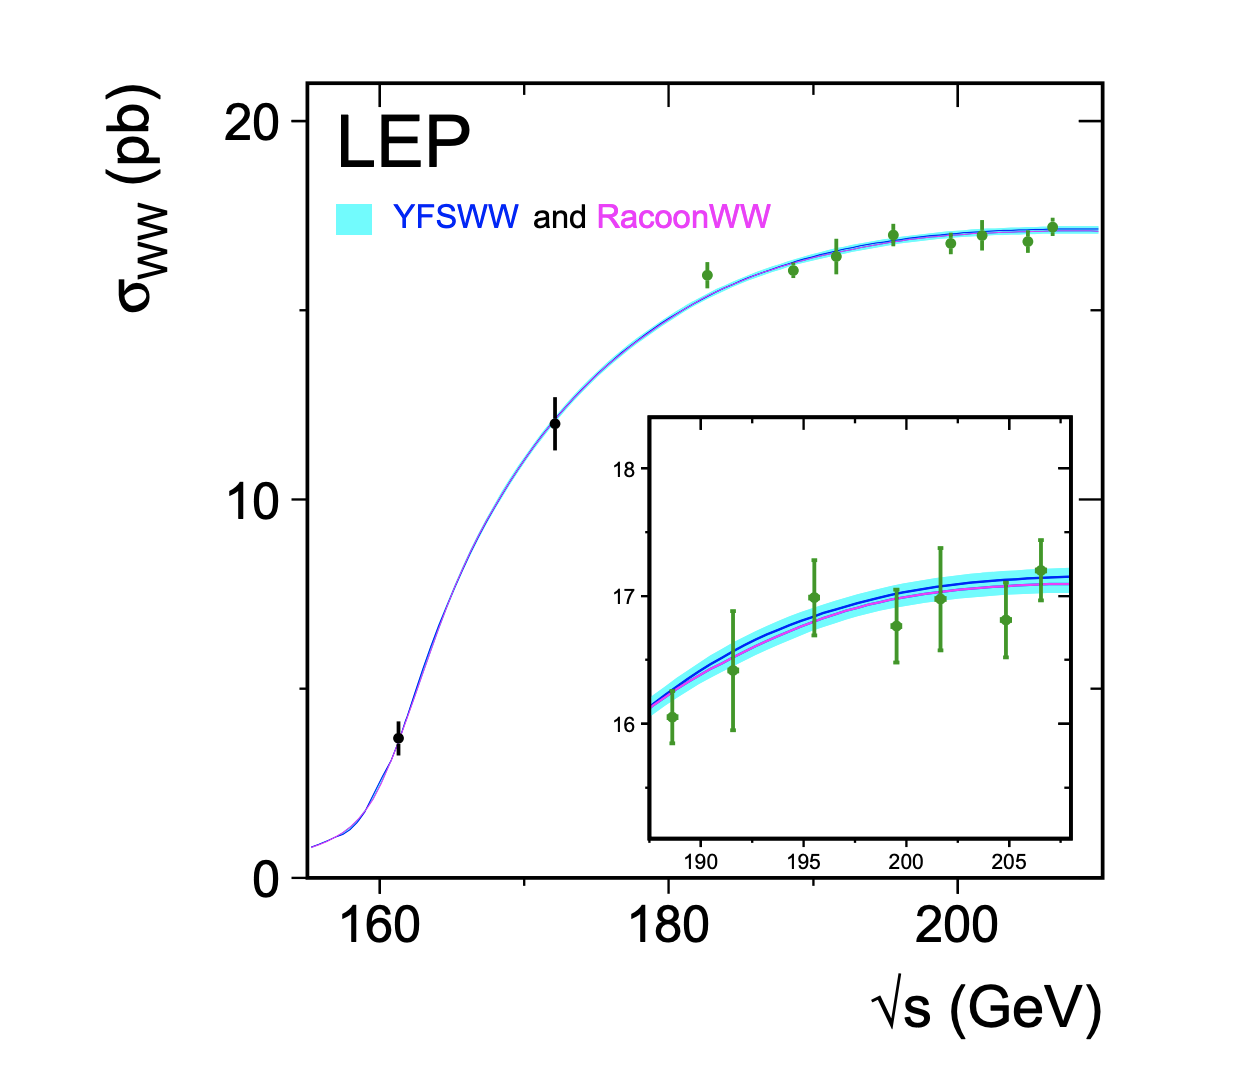
\includegraphics[width=0.59\textwidth]{chapters/introduction/sectionRelatedWorks/figures/lepCrosssection.png}
    \caption{The LEP measurement of \WW production cross-section. The measurement was a combine of the four LEP experiments, with a total 3\fbinv  data. The \WW production at LEP was mainly induced by exchanging neutrinos in the t-channel and quark annihilation to $\PZ/\gamma$  in the s-channel. The measured cross-section agreed with the theoretical calculation.}
    \label{fig:introduction:relatedWorks:lepCrosssection}
\end{figure}


The LEP at CERN collided electrons and positrons at the center-of-mass energy of \PZ pole during its first running phase (1989-1995). Then the collision energy was increased to a maximum of 209\GeV during its second running phase (LEP-2 1995-2000). In some parts of 1995 and 1997, LEP was operated at center-of-mass energies below the \WW resonance at 130.3\GeV, 136.3\GeV, and 140.2\GeV. The rest runs of LEP-2 scanned at ten different energies above the \WW resonance ranging in 161.3 - 209\GeV. During the full scanning the center-of-mass energy from 130\GeV to 209\GeV, the four LEP experiments ALEPH, DELPHI, L3, and OPAL, collected a total data of 3\fbinv integrated luminosity. 

ALEPH was a cylindrical symmetric detector with a tracking system  (drift chamber and TPC) and electromagnetic calorimeter, supper conducting solenoid, streamer tubes inserted in the iron return yokes for the hadron and muon detection. DELPHI was also a cylindrical general-purpose detector consisting of vertex detector, time projection chamber (TPC) tracker, Ring-Imaging Cherenkov detector, electromagnetic calorimeter, solenoid, hadroinc calorimeter, muon chamber. OPAL's structure was formed by vertex detector, tracker, magnetic solenoid, crystal ECAL/HCAL, and muon detector. Unlike the other 3 detectors, L3 had its magnetic solenoid as the outmost layer; inside were trackers (silicon strip micro vertex detector and time expansion chamber), electromagnetic/hadronic calorimeters, and muon chamber. 

The \WW production in the electron positron collision was primarily induced by the electroweak process in the t-channel exchanging $\PGn_\Pe$, and the triple gauge boson coupling process in the s-channel mediated by \PZ boson or photon. The measurement of \WW production cross-section from the four LEP experiments combined is shown in Figure~\ref{fig:relatedWorks:lu:W:lepWWxs}. There is a clear turn-on for the \WW production at the 161.3 GeV. The combined result of \WW cross-section is consistent with the theoretic prediction by YFSWW and RACOONWW.


% LEP result plot
\begin{figure}[ht]
    \centering
    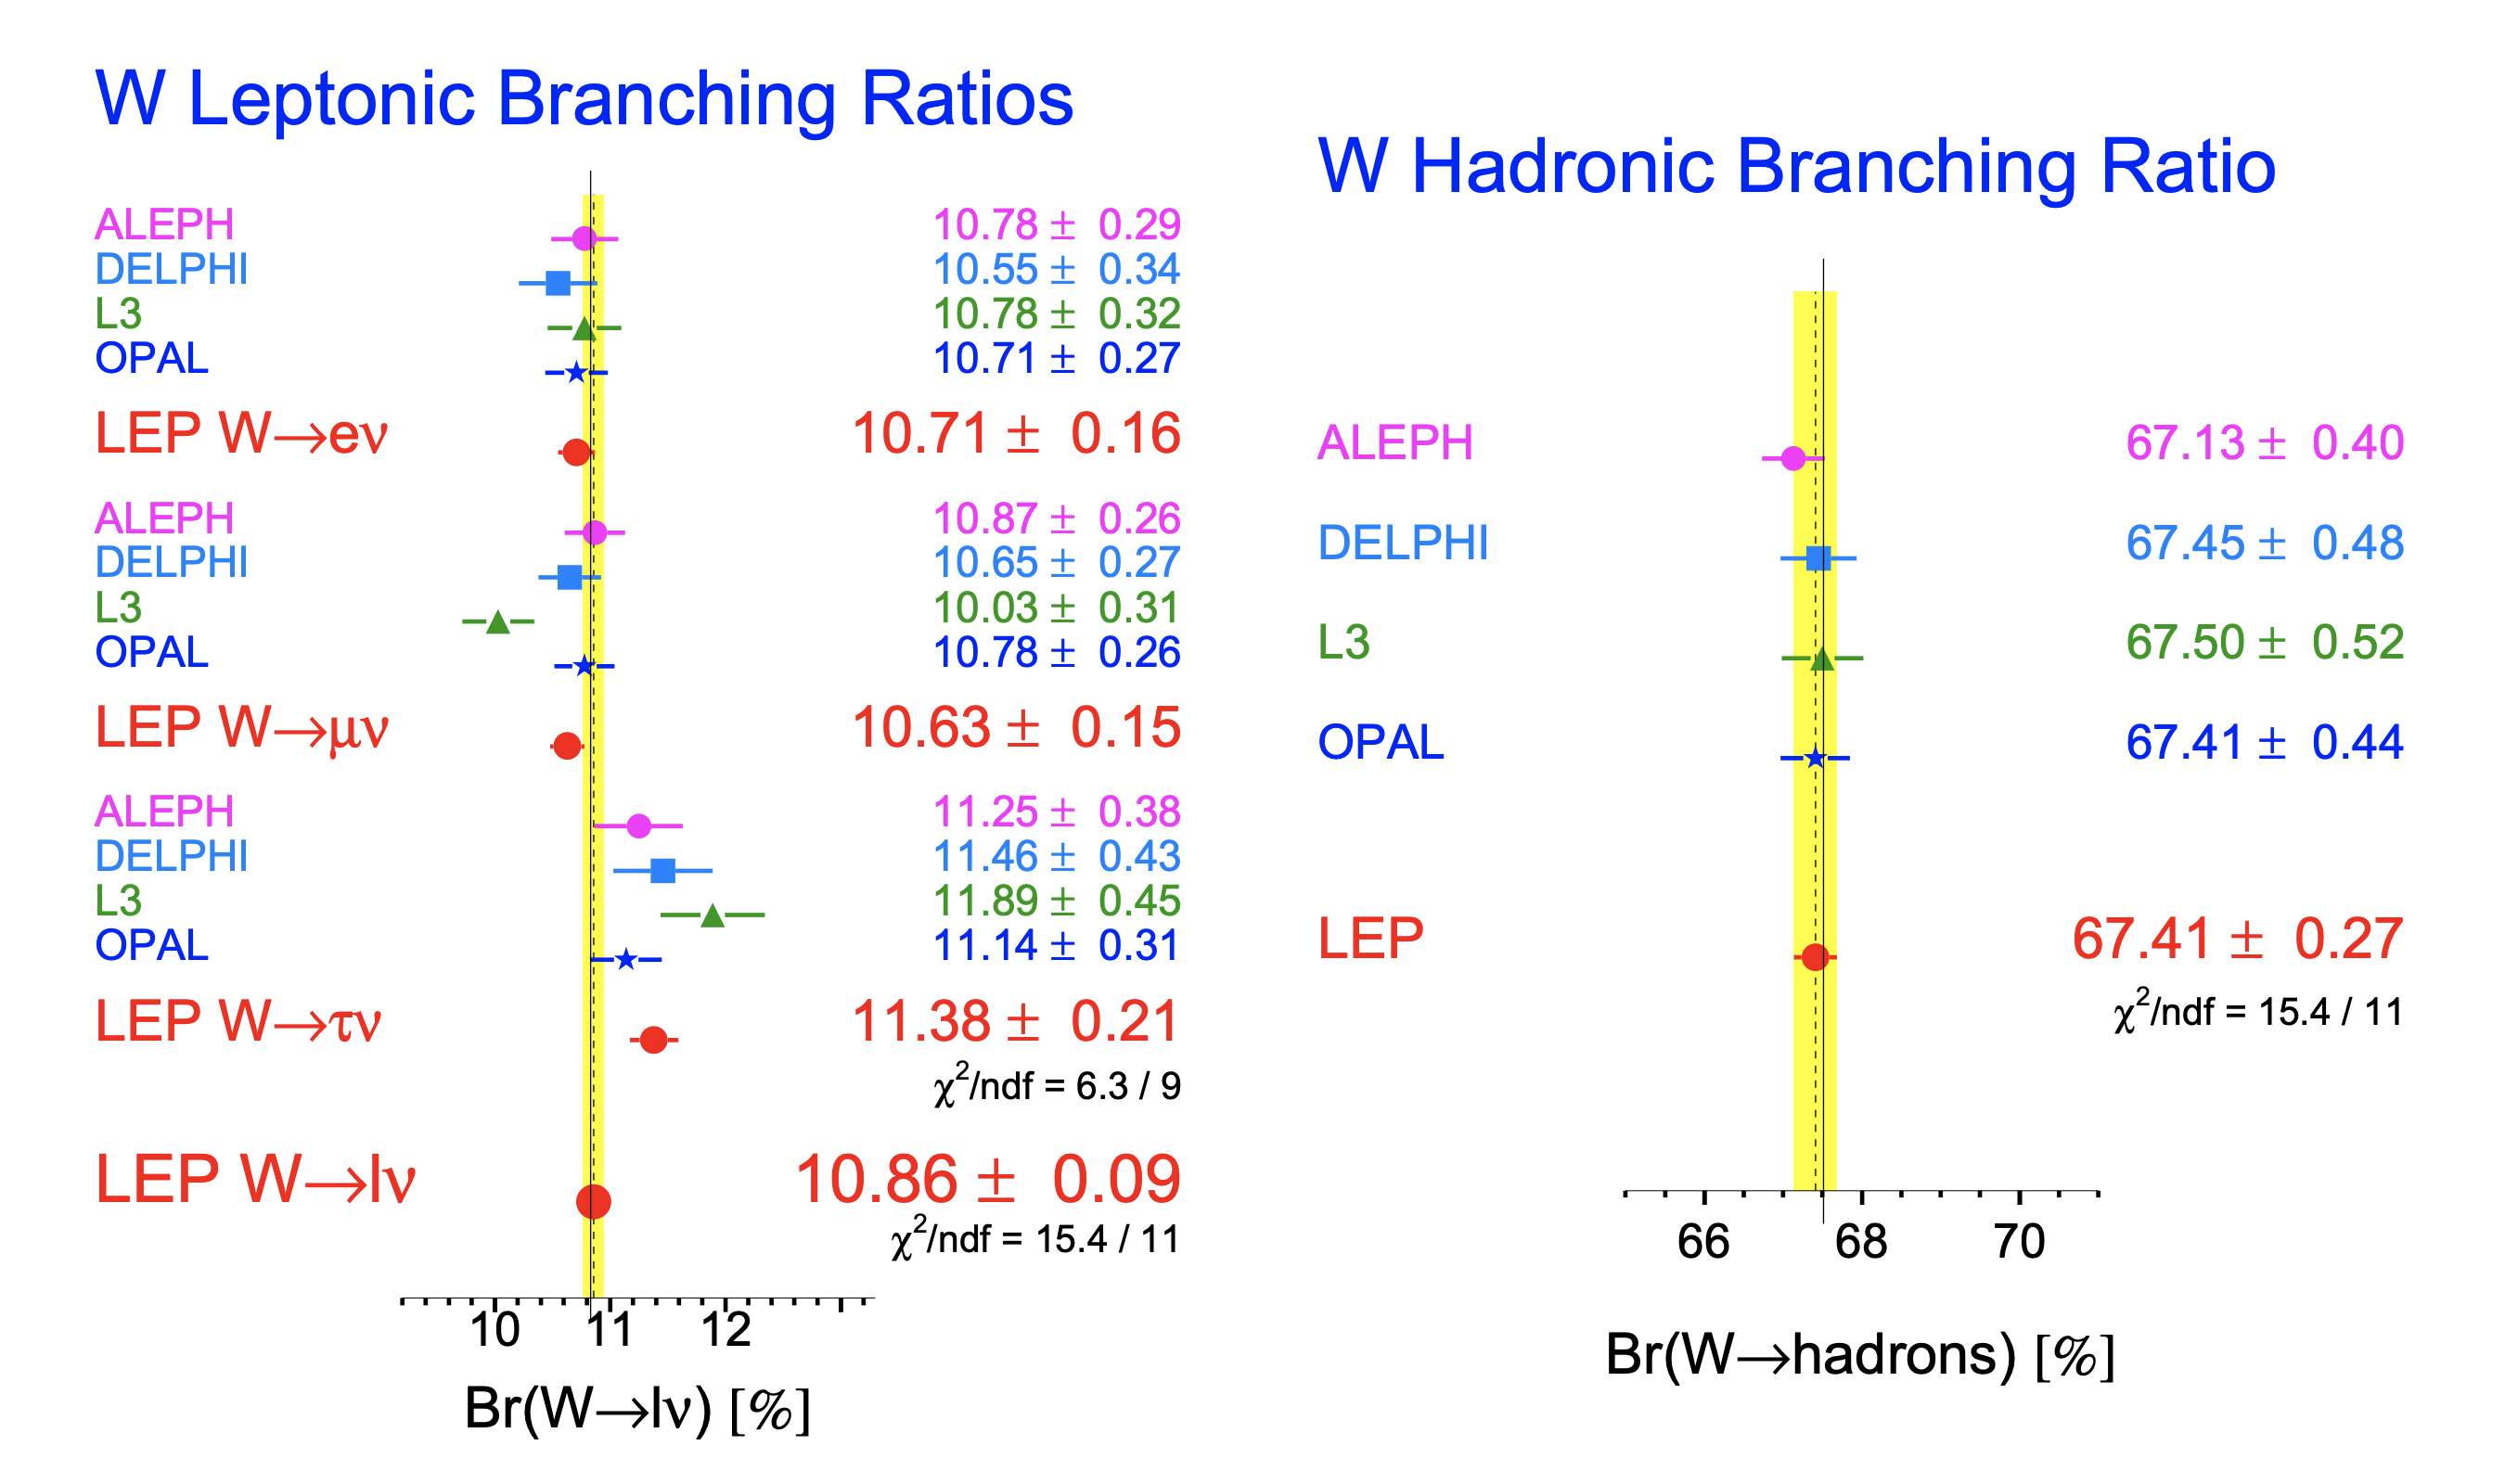
\includegraphics[width=0.99\textwidth]{chapters/introduction/sectionRelatedWorks/figures/lep.png}
    \caption{\PW leptonic and hadronic branching fractions from the four LEP experiments \cite{Schael:2013ita}. }
    \label{fig:introduction:relatedWorks:lep}
\end{figure}


Each experiment determined the three \PW leptonic decay branching fractions from the \WW cross-sections measurement \cite{Schael:2013ita}. The hadronic branching fraction was determined from the leptonic ones based on the unitarity. When combining the four experiments, the theoretical uncertainties of signal and background, as well as the theoretical uncertainties of the luminosity, were treated as correlated; the experimental uncertainties on the luminosity, detector effects, and simulation statistics are treated as uncorrelated. The details of the \BWl results and the correlations are summarized in Table~\ref{tab:relatedWorks:lu:W:lep} and in Figure~\ref{fig:relatedWorks:lu:W:lep}. A suspicious excess of the lepton universality was observed in the result. While the electronic and muonic branching fractions agree well with each other, the tauonic branching fraction is significantly larger than the average of the other two. The ratio between the \BWt and the average of \BWe and \BWm was reported as \cite{Schael:2013ita} $1.066 \pm 0.025$, showing a 2.6 standard deviation from the lepton universality.


% LEP result table
\begin{table}[!ht]
    \setlength{\tabcolsep}{.5 em}
    \renewcommand{\arraystretch}{1.5}
    \centering
    \caption{Three individual leptonic branching fractions from the four LEP experiments and the combined result \cite{Schael:2013ita}.}
    % \resizebox{\textwidth}{!}{
    \begin{tabular}{ |c| c  c | } 
         %  LEP ALEPH
         \hline
         \multicolumn{3}{|c|}{ALEPH \cite{Heister:2004wr}} \\
         \hline
         \BWe    & 10.78 $\pm$ 0.27 (stat) $\pm$ 0.10 (syst) & 
         \multirow{3}{*}{
            \begin{footnotesize}
            $\begin{bmatrix}
                +1.000 &-0.009 &-0.332 \\ 
                -0.009 &+1.000 &-0.268 \\
                -0.332 &-0.268 &+1.000 
            \end{bmatrix}$ 
            \end{footnotesize} 
         } \\
         \BWm    & 10.87 $\pm$ 0.25 (stat) $\pm$ 0.08 (syst) & \\ 
         \BWt    & 11.25 $\pm$ 0.32 (stat) $\pm$ 0.20 (syst) & \\
         \hline
         \multicolumn{3}{c}{} \\
         
         
         %  LEP DELPHI
         \hline
         \multicolumn{3}{|c|}{DELPHI \cite{Abdallah:2003zm}} \\
         \hline
         \BWe    & 10.55 $\pm$ 0.31 (stat) $\pm$ 0.14 (syst) & 
         \multirow{3}{*}{
            \begin{footnotesize}
            $\begin{bmatrix}
                +1.000 &+0.030 &-0.340 \\ 
                +0.030 &+1.000 &-0.170 \\
                -0.340 &-0.170 &+1.000 
            \end{bmatrix}$ 
            \end{footnotesize} 
         } \\
         \BWm    & 10.65 $\pm$ 0.26 (stat) $\pm$ 0.08 (syst) & \\ 
         \BWt    & 11.46 $\pm$ 0.39 (stat) $\pm$ 0.19 (syst) & \\
         \hline
         \multicolumn{3}{c}{} \\
         
         
         %  LEP L3
         \hline
         \multicolumn{3}{|c|}{L3 \cite{Achard:2004zw}} \\
         \hline
         \BWe    & 10.78 $\pm$ 0.29 (stat) $\pm$ 0.13 (syst) & 
         \multirow{3}{*}{
            \begin{footnotesize}
            $\begin{bmatrix}
                +1.000 &+0.136 &-0.201 \\ 
                +0.136 &+1.000 &-0.122 \\
                -0.201 &-0.122 &+1.000 
            \end{bmatrix}$ 
            \end{footnotesize} 
         } \\
         \BWm    & 10.03 $\pm$ 0.29 (stat) $\pm$ 0.12 (syst) & \\ 
         \BWt    & 11.89 $\pm$ 0.40 (stat) $\pm$ 0.20 (syst) & \\
         \hline
         
         \multicolumn{3}{c}{} \\
         
         %  LEP OPAL
         \hline
         \multicolumn{3}{|c|}{OPAL \cite{Abbiendi:2007rs}} \\
         \hline
         \BWe    & 10.71 $\pm$ 0.25 (stat) $\pm$ 0.11 (syst) & 
         \multirow{3}{*}{
            \begin{footnotesize}
            $\begin{bmatrix}
                +1.000 &+0.135 &-0.303 \\ 
                +0.135 &+1.000 &-0.230 \\
                -0.303 &-0.230 &+1.000 
            \end{bmatrix}$ 
            \end{footnotesize} 
         } \\
         \BWm    & 10.78 $\pm$ 0.24 (stat) $\pm$ 0.10 (syst) & \\ 
         \BWt    & 11.14 $\pm$ 0.31 (stat) $\pm$ 0.17 (syst) & \\
         \hline
         
         \multicolumn{3}{c}{} \\
         %  LEP Average
         \hline
         \multicolumn{3}{|c|}{LEP Average \cite{Schael:2013ita}} \\
         \hline
         \BWe    & 10.71 $\pm$ 0.14 (stat) $\pm$ 0.07 (syst) & 
         \multirow{3}{*}{
            \begin{footnotesize}
            $\begin{bmatrix}
                +1.000 &+0.136 &-0.201 \\ 
                +0.136 &+1.000 &-0.122 \\
                -0.201 &-0.122 &+1.000 
            \end{bmatrix}$ 
            \end{footnotesize} 
         } \\
         \BWm    & 10.63 $\pm$ 0.13 (stat) $\pm$ 0.07 (syst) & \\ 
         \BWt    & 11.38 $\pm$ 0.17 (stat) $\pm$ 0.11 (syst) & \\
         \hline
        %  *$Br(W\to \mu  \nu)/ Br(W\to e \nu)$ & 0.993  $\pm$ 0.019 & 
        %  \multirow{3}{*}{
        %     \begin{footnotesize}
        %     $\begin{bmatrix}
        %         +1.000 &+0.440 &-0.314 \\ 
        %         +0.440 &+1.000 &+0.714 \\
        %         -0.314 &+0.714 &+1.000 
        %     \end{bmatrix}$ 
        %     \end{footnotesize} 
        %  } \\
        %  *$Br(W\to \tau \nu)/ Br(W\to e \nu)$ & 1.063  $\pm$ 0.027 & \\
        %  *$Br(W\to \tau \nu)/ Br(W\to\mu\nu)$ & 1.070  $\pm$ 0.026 &  \\
         
        %  \hline
    \end{tabular}
    % }
    \label{tab:introduction:relatedWorks:lep}
\end{table}




\FloatBarrier
\underline{LHC}

During the LHC run-1 at a center-of-mass energy of 7 TeV and 8 TeV, the lepton universality was studied in the electron and muon channels of \wjets events. Two such measurements were published by the ATLAS and LHCb. ATLAS measured the $\sigma_{\Pp\Pp \to \PW} \times \BWem$ \cite{Aaboud:2016btc} with 7\TeV data collected in 2011 corresponding to 4.6\fbinv integrated luminosity. The events were triggered with single-lepton triggers and selected with several lepton isolation and identification cuts, as well as \MET cuts. The ratio $\frac{ \BWm }{ \BWe}$ was determined as $1.003\pm 0.010$. LHCb measured the $\sigma_{\Pp\Pp \to \PW} \times \BWe$ \cite{Aaij:2016qqz} and $\sigma_{\Pp\Pp \to \PW} \times \BWm$ \cite{Aaij:2015zlq} in two separate analysis with 8 TeV data corresponding to 2\fbinv integrated luminosity. The events were also triggered with the single-lepton triggers, and the selections required on lepton quality and \MET. To test universality, the second analysis \cite{Aaij:2016qqz} compared its electron channel to the muon channel published in the first analysis \cite{Aaij:2015zlq}, taking into account the experimental correlations. The comparison included both the total cross-section and the differential cross-section with respect to pseudorapidity. The differential cross-section agreed well between the electron channel and muon channel. Their ratio led to $\frac{ \BWm }{ \BWe}  = 0.980 \pm 0.018 $.


During the LHC run-2 at a center-of-mass energy of 13\TeV, \PW bosons from the \ttbar events are treated as the major signal for the LU test, thanks to the high \ttbar cross-section at 13\TeV. ATLAS~\cite{Aad:2020ayz} measured the ratio between the tauonic and the muonic branching fractions $\frac{ \BWt }{ \BWm} $ using the LHC run-2 data at 13 TeV collected during 2016-2018 corresponding to 139\fbinv integrated luminosity. The analysis selects \ttbar events with a single-muon trigger and applies additional requirements on muon quality, jet multiplicity, and \PQb tag multiplicity for a \ttbar-enriched sample. Tau is probed with tau's muonic decay, which is about 17\% of the total tau decay width. The measurement fits to the distribution of the impact parameter of the selected muons to discriminate $\PW \to \PGm$ and $\PW \to \PGt \to \PGm$. Probing taus with their muonic decay helps cancel the systematical uncertainties related to the muon reconstruction. Also, the systematical uncertainties concerning hadronic tau identification is avoided. The reported result of the branching ratio is

$$ \frac{ \BWt }{ \BWm} = 0.992 \pm 0.013 \text{ (ATLAS) }$$





\subsubsection{Test with Meson Decay}


% meson decay table
\begin{table}[ht]
    \setlength{\tabcolsep}{.5 em}
    \renewcommand{\arraystretch}{1.5}
    \centering
    \caption{SM prediction and the experimental measurements of the leptonic or semi-leptonic branching ratios of the pseudoscalar mesons. \cite{Bifani:2018zmi} }
    \resizebox{\textwidth}{!}{
    \begin{tabular}{|c|c|c|c|}
        \hline
         & SM Prediction & World Average & Included measurements \\
        \hline
        % pi
        $R^\pi_{\Pe/\mu} \; [10^{-4}]$ &  1.2352 $\pm$ 0.0001 \cite{Cirigliano:2007xi} & 1.2327 $\pm$ 0.0023  & 
            \tiny{ TRIUMF \cite{Numao:1992ve, Britton:1992pg}, PiENu \cite{Aguilar-Arevalo:2015cdf}, BGO-OD \cite{Czapek:1993kc}} \\
        % K
        $R^K_{\Pe/\mu} \; [10^{-5}]$ &  2.477  $\pm$ 0.001 \cite{Cirigliano:2007xi} & 2.488  $\pm$ 0.009 & 
            \tiny{NA62 \cite{Lazzeroni:2012cx}, KLOE \cite{Ambrosino:2009aa} }\\
        % D_s
        $R^{D_s}_{\tau/\mu} $ &  9.76 $\pm$ 0.10 \cite{Dobrescu:2008er} & 9.95 $\pm$ 0.61  & 
            \tiny{ HFLAV \cite{Amhis:2016xyh} ave of CLEO, BASIII, BELLE, BABAR} \\
        
        \hline
        % B D
        $R^{B}_{D, \tau/l} $ &  0.299  $\pm$ 0.003  \cite{Bifani:2018zmi} & 0.340  $\pm$ 0.030 & 
            \tiny{BABAR \cite{Lees:2012xj, Lees:2013uzd}, Belle \cite{Huschle:2015rga} }\\
            
        % B D*
        $R^{B}_{D*, \tau/l} $ &  0.258  $\pm$ 0.005 \cite{Bifani:2018zmi} & 0.295  $\pm$ 0.014 & 
            \tiny{BABAR \cite{Lees:2012xj, Lees:2013uzd}, Belle \cite{Huschle:2015rga, Sato:2016svk, Hirose:2016wfn}, LHCb\cite{Aaij:2015yra,Aaij:2017uff, Aaij:2017deq} }\\
            
        \hline
    \end{tabular}}
    \label{tab:introduction:relatedWorks:meson}
\end{table}

The charged weak current decays of mesons mediated by \PW bosons also provide tests of LU.  The most stringent constraints come from the study of fully-leptonic decay of the charged pions or kaons, which are helicity suppressed in the SM depending on the lepton mass. Pions and kaons are kinematically allowed to decay into electrons and muons. The ratio between the electronic and muonic branching fractions of pion is measured by TRIUMF \cite{Numao:1992ve, Britton:1992pg}, PiENu \cite{Aguilar-Arevalo:2015cdf} and BGO-OD\cite{Czapek:1993kc},  while that of kaon is measured by NA62 \cite{Lazzeroni:2012cx} and KLOE \cite{Ambrosino:2009aa}, shown in Table~\ref{tab:introduction:relatedWorks:meson}. The measured ratios are consistent with the SM LU predictions. For \PDs meson, tauonic decay is possible, and the ratio between tauonic and muonic branching fraction $R^\PDs_{\PGt/\PGm}$ is measured in the charm factories including CLEO, BASIII, Belle, and BaBar. Table~\ref{tab:introduction:relatedWorks:meson} shows these experimental measurements and the comparison to the SM theoretical calculations, where the agreement to LU is indicated. 

Additionally, the tests of LU can be performed by taking ratios between the semi-leptonic charged weak decays of mesons, such as $\PD\to \PK \ell\PGn$. Heavy Flavor Averaging Group (HGLAV) \cite{Amhis:2019ckw} provides a summary of the LU test using the semi-leptonic charged weak decays of the \PD meson and the \PB meson. An anomaly is observed in the $\PB\to \PD^{(*)} \ell\PGn$ semi-leptonic decay in the tau channel versus the electron and muon channel. $R^{B}_{D^{(*)}, \PGt/l}$ is measured in the Belle \cite{Huschle:2015rga, Sato:2016svk, Hirose:2016wfn}, BaBar  \cite{Lees:2012xj, Lees:2013uzd} and LHCb \cite{Aaij:2015yra,Aaij:2017uff, Aaij:2017deq}. Ratios are defined as $R^{\PB}_{\PD^{(*)}, \PGt/\ell} = \frac{Br(\PB\to \PD^{(*)} \PGt \PGn)}{Br(\PB\to \PD^{(*)}  \ell \PGn)}$ where $\ell=\Pe,\PGm$. The experimental results are listed in Table~\ref{tab:introduction:relatedWorks:meson}. Figure~\ref{fig:introduction:relatedWorks:bmeson} illustrates this anomaly in the \PB meson semi-leptonic decays. The world average of Belle, BaBar and LHCb is about four sigma deviated from the SM theoretical prediction.

% However, these tests require knowledge of the ratio of the form factors of the scalar and vector meson, f0/f+, with very high accuracy to be competitive with the leptonic decays, where the main hadronic input (meson decay constants) drops out of the LU ratios. 



% B meson decay plot
\begin{figure}[ht]
    \centering
    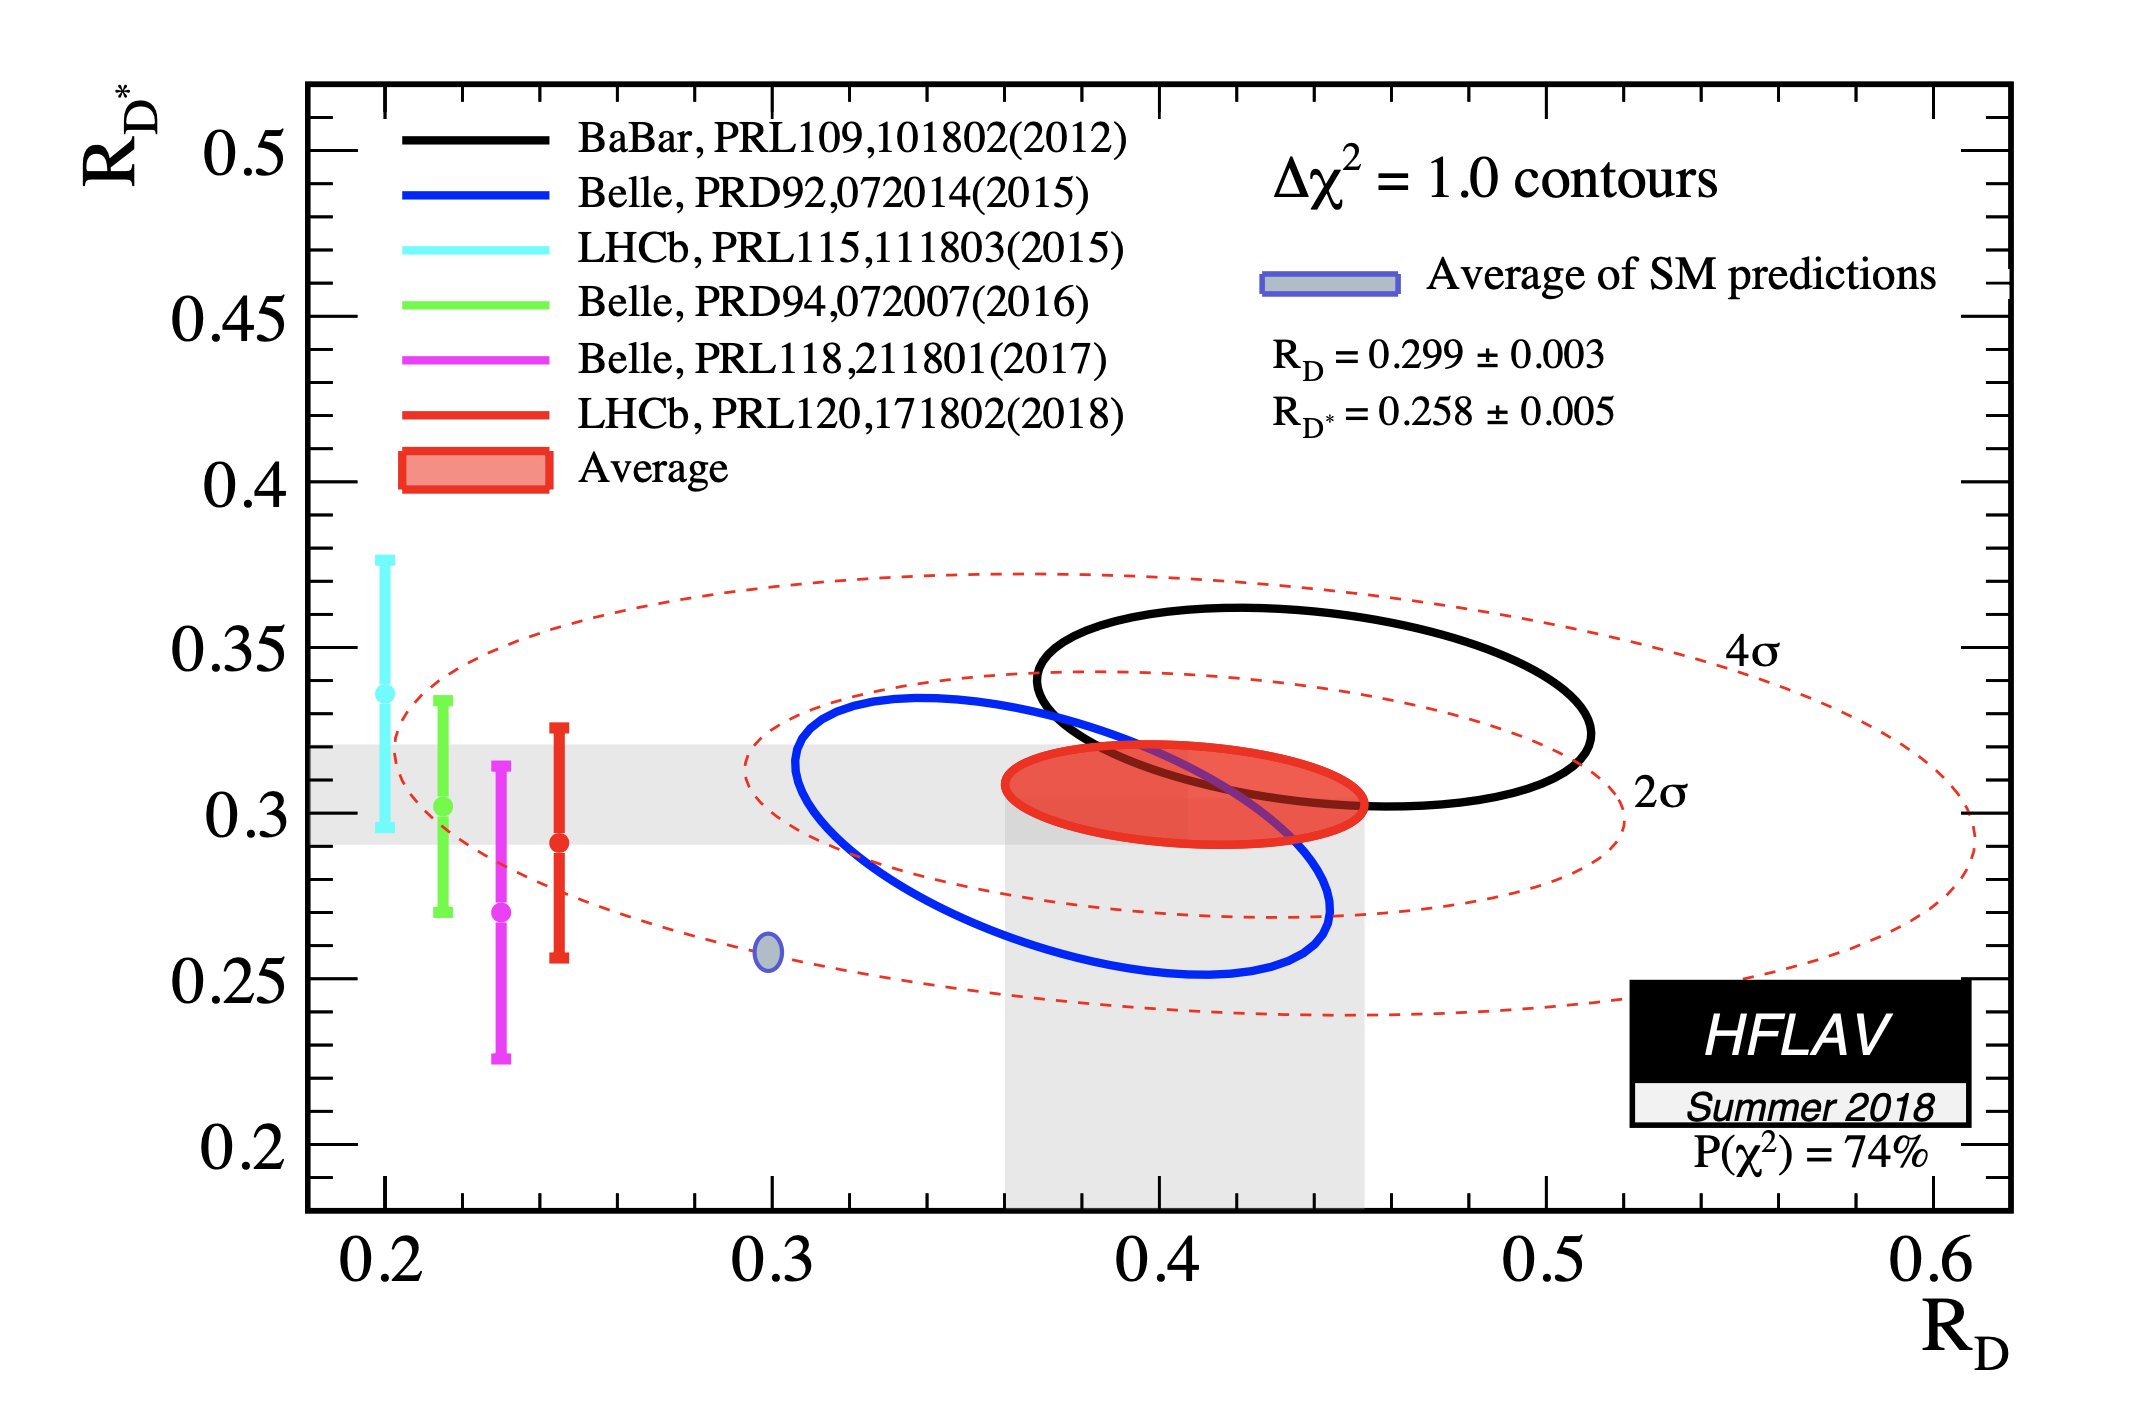
\includegraphics[ width = 0.7 \textwidth ]{chapters/introduction/sectionRelatedWorks/figures/bmeson.png}
    \caption{ Anomaly of lepton universality in the semi-leptonic decays of \PB meson \cite{Amhis:2019ckw}. The world average of $R^{B}_{D, \PGt/l}$  and $R^{B}_{D^*, \PGt/l}$  shows a four sigma deviation from the SM prediction.}
    \label{fig:introduction:relatedWorks:bmeson}
\end{figure}




\subsubsection{Test with Tau Decay}


The LU involving the charged weak current can also be tested by the tau precision measurements \cite{Pich:2013lsa,Amhis:2019ckw}. In the SM, the only expected difference between $\PGt^- \to e^- \bar{\PGn}_\Pe \PGn_\PGt$ and $\PGt^- \to \PGm^- \bar{\PGn}_\PGm \PGn_\PGt$  decay is due to the decay kinematic phase space. $g_\PGm  / g_\Pe $ can be obtained by precision measurements of tau's electronic and muonic decay widths. Similarly,  $g_\PGt  / g_\PGm $ can be obtained by precision measurement of tau's electronic decay $\PGt^- \to e^- \bar{\PGn}_\Pe \PGn_\PGt$ and muon's electronic decay $\PGm^- \to e^- \bar{\PGn}_\Pe \PGn_\PGm$.  The ratio of the weak couplings to the third and first generation leptons can be obtained from the measurements of the width of $\PGt^- \to \PGm^- \bar{\PGn}_\PGm \PGn_\PGt$  and $\PGm^- \to e^- \bar{\PGn}_\Pe \PGn_\PGm$.  These represent one of the most stringent experimental tests for LU in the electroweak sector. By global fitting to the tau precision measurements, HFLAV~\cite{Amhis:2019ckw} determines the ratios of electroweak coupling constant among the three leptons as 

\begin{align*}
    g_\PGt / g_\PGm &= 1.0010 \pm 0.0014 \\
    g_\PGt / g_\Pe   &= 1.0029 \pm 0.0014 \\
    g_\PGm  / g_\Pe   &= 1.0018 \pm 0.0014 
\end{align*}



\subsection{Measurements of $\mathrm{V}_{cs}$ }
\label{sec:introduction:relatedWorks:vcsMeasurements}

The CKM matrix represents the mixing between quarks' mass eigenstates and the flavor eigenstates. When physical quarks in their mass eigenstates participate in the weak interaction, they are projected to the flavor eigenstates by the CKM matrix. More details about the CKM in the standard model are discussed in Appendix~\ref{sec:relatedWorks:qft:gws}. 

\begin{table}[ht]
    \centering
    \setlength{\tabcolsep}{1.5em}
    \renewcommand{\arraystretch}{1.5}
    \caption{The world average of the experimental measurements of the nine elements in the CKM matrix in the PDG \cite{pdg2020}.  }
    \resizebox{\textwidth}{!}{
    \begin{tabular}{c|c|c }
        \hline
        $\absVud=0.97370 \pm 0.00014 $     & $\absVus=0.2245 \pm 0.0008$      &  $\absVub=0.00382 \pm 0.00024$   \\ \hline
        $\absVcd=0.221 \pm 0.004 $         & $\absVcs=0.987 \pm 0.011$        &  $\absVcb=0.0410 \pm 0.0014$     \\ \hline
        $\absVtd=0.0080 \pm 0.0003 $       & $\absVts=0.0388 \pm 0.0011$      &  $\absVtb=1.013 \pm 0.030$       \\
        \hline
    \end{tabular}}
    \label{tab:introduction:relatedWorks:ckm}
\end{table}


The current experimental measurements of the nine elements in the CKM matrix \cite{pdg2020} are shown in Table~\ref{tab:introduction:relatedWorks:ckm}. Among the six elements in the first two rows, the measurement of \absVcs shown in Figure~\ref{fig:introduction:relatedWorks:vcs} has the least precision. Currently, there are two direct approaches to measure \absVcs, using the \PD meson decay in the charm factories and using the on-shell $\PW\to c s$  with jet tagging in the collider experiments.

The best direct determination of \absVcs is from the semi-leptonic decay of \PD meson and the leptonic decay of \PDs meson produced in the charm factory. For \PDs meson, the branching fraction of $\PDs^+ \to \PGm^+ \PGn$ and $\PDs^+ \to \PGt^+ \PGn$ are both measured in the Belle \cite{Zupanc:2013byn}, CLEO \cite{Alexander:2009ux,Onyisi:2009th,Naik:2009tk}, BaBar \cite{delAmoSanchez:2010jg} and BESIII \cite{Ablikim:2016duz, Ablikim:2018jun}. Using the experimental value of the mass and lifetime of \PDs meson, as well as the lattice QCD calculation of the form factor $f_{\PDs}$, \absVcs can be determined from the \PDs leptonic decay and yields a world average of $\absVcs=0.992\pm 0.012$ \cite{Amhis:2019ckw}, where the dominating uncertainty is from the experimental error. For \PD meson, the branching fraction of $\PD\to \PK \ell\PGn$ is measured by CLEO-c \cite{Besson:2009uv}, Belle \cite{Widhalm:2006wz}, BaBar \cite{Aubert:2007wg} and BESIII \cite{Ablikim:2015ixa, Ablikim:2018evp}, which leads to an average of \absVcs of $\absVcs=0.939\pm 0.038$ \cite{Amhis:2019ckw} in the \PD meson decay. The dominant uncertainty is form the theoretical calculations of the \PD meson form factor with latice QCD. Combining the results from the \PD and \PDs meson decays, the charm factories produce $\absVcs=0.987\pm 0.011$ \cite{Amhis:2019ckw}. This is also the value considered as the world average by the PDG~\cite{pdg2020}.

The second direct measurement of \absVcs is from the on-shell $\PW\to \PQc \PQs$ decays in the collider experiments. This approach relies on jet tagging to identifies the jets originating from the \PQc and \PQs quarks, which is relatively difficult, especially in the LHC with a more complex hadron environment. Therefore, this approach is less explored comparing with the $\PD/\PDs$ approach. So far, the only published result based on the $\PW\to \PQc \PQs$  approach is from the DELPHI~\cite{Abreu:1998ap} in the LEP. DELPHI identified the charged mesons based on their ionization energy losses while traversing through the TPC tracking system. Since \PQs and \PQc jets tend to include energetic kaons, they were first tagged by the \pt and the particle identity ($\pi$ or \PK) of the leading meson in the jet. Then the impact parameters of the tracks in the jet were considered to discriminate \PQc quark jets against other jets. The result from DELPHI was reported as $\absVcs=0.94 ^{+0.32}_{-0.26}\pm 0.13$. 

In addition, LEP published one indirect result. LEP measures the $\BWl = (10.83 \pm 0.07 \pm 0.07) \%$ \cite{Schael:2013ita}, based on which calculates the sum of all six CMK element in the first two rows as $\sumCKM = 2.002 \pm 0.027$. Since \absVcs is the least precisely measured element, LEP subtract other five elements from \sumCKM and produces an indirect measurement of $\absVcs=0.969\pm 0.013$. With the latest CKM values for the other five elements, repeating LEP's calculation gives $\absVcs=0.972\pm 0.013$. The same calculation can be done with the \BWl measurement by the CMS presented in this thesis.


 \begin{figure}
    \centering
    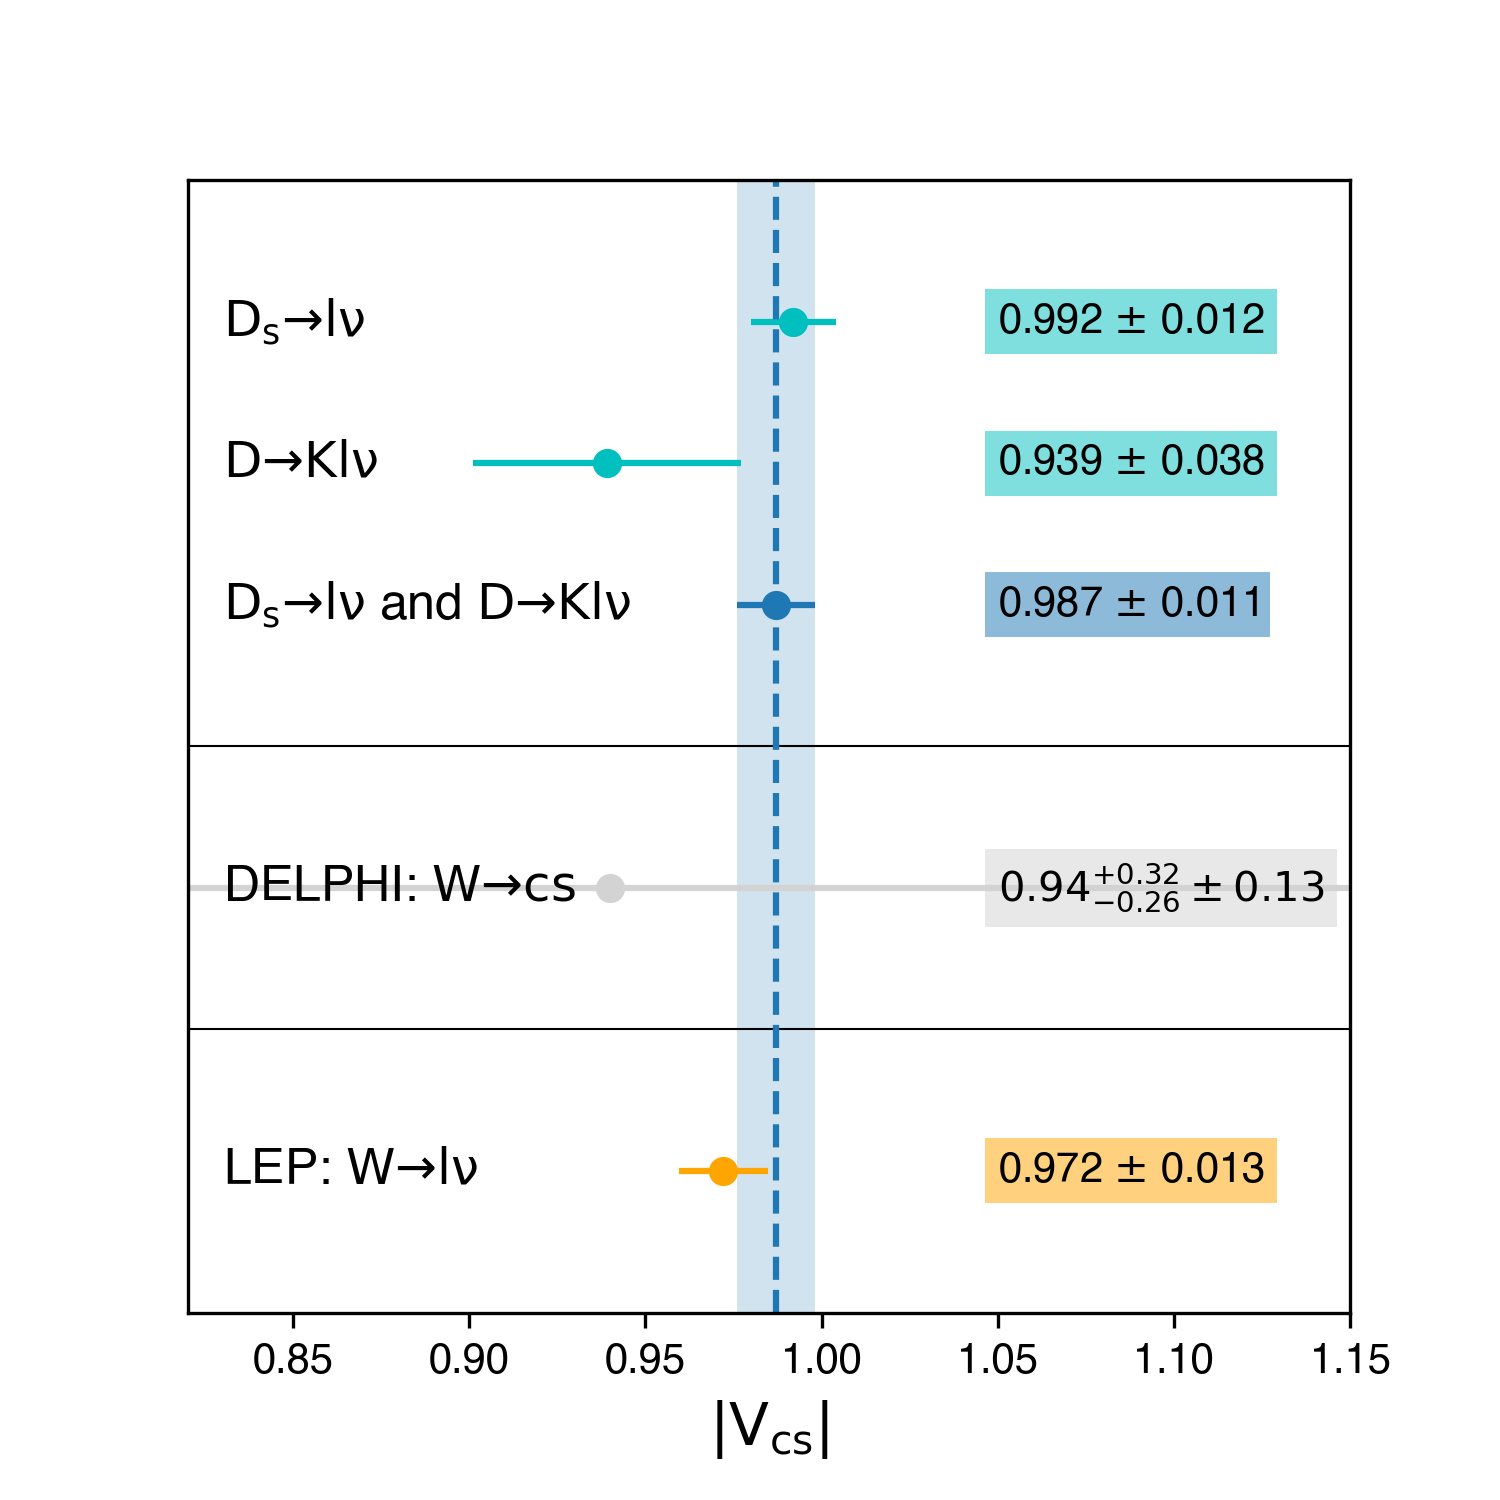
\includegraphics[width=0.6\textwidth]{chapters/introduction/sectionRelatedWorks/figures/vcs0.png}
    \caption{The \absVcs measurements~\cite{pdg2020}. The 2020 PDG average~\cite{pdg2020} combines the results from \PD and \PDs decay.}
    \label{fig:introduction:relatedWorks:vcs}
\end{figure}
